
\section{Ausgangsleistung}
\label{section:ausgangsleistung}
\begin{frame}%STARTCONTENT

\begin{columns}
    \begin{column}{0.48\textwidth}
    \begin{itemize}
  \item Klasse~N ist in Strahlungsleistung (ERP oder EIRP) an Antenne begrenzt
  \end{itemize}

    \end{column}
   \begin{column}{0.48\textwidth}
       \begin{itemize}
  \item Klassen E und A meistens auf \emph{Senderausgangsleistung} (peak envelope power, PEP)
  \end{itemize}

   \end{column}
\end{columns}
    \pause
    \begin{itemize}
  \item Viele Funkgeräte zeigen die aktuelle Senderausgangsleistung im Power-Meter an.
  \end{itemize}


\end{frame}

\begin{frame}
\only<1>{
\begin{PQuestion}{NF102}{Die Darstellung zeigt das Display eines Transceivers. Wie wird die Anzeige 2 im Sendebetrieb bezeichnet?}{Power-Meter}
{Amplitudenspektrum}
{SWR-Meter}
{Wasserfalldiagramm}
{\DARCimage{1.0\linewidth}{578include}}\end{PQuestion}

}
\only<2>{
\begin{PQuestion}{NF102}{Die Darstellung zeigt das Display eines Transceivers. Wie wird die Anzeige 2 im Sendebetrieb bezeichnet?}{\textbf{\textcolor{DARCgreen}{Power-Meter}}}
{Amplitudenspektrum}
{SWR-Meter}
{Wasserfalldiagramm}
{\DARCimage{1.0\linewidth}{578include}}\end{PQuestion}

}
\end{frame}

\begin{frame}
\frametitle{Zulässige Senderausgangsleistung}
\begin{itemize}
  \item In Anlage 1 der AFuV
  \item Unterscheidet sich je nach Klasse und Frequenzbereich
  \end{itemize}

\end{frame}

\begin{frame}
\begin{figure}
    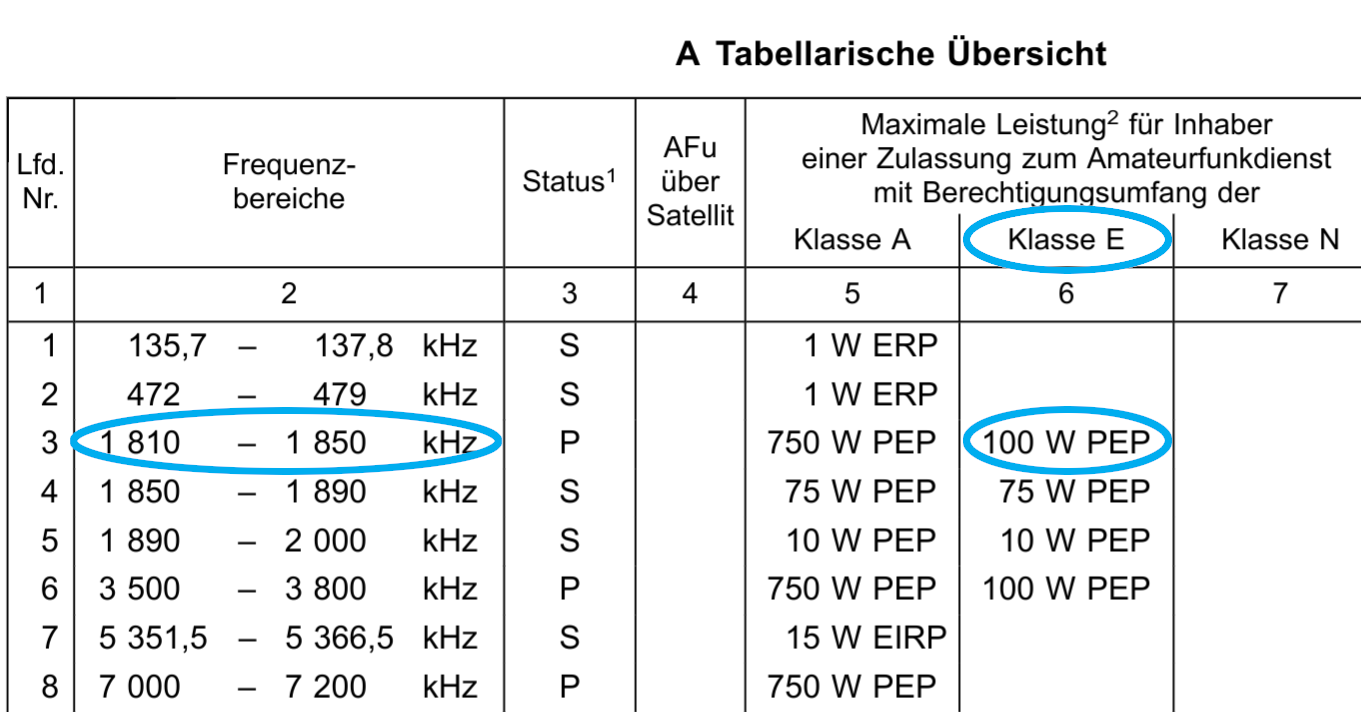
\includegraphics[width=0.85\textwidth]{foto/145}
    \caption{\scriptsize Ausschnitt aus der Anlage 1 der Amateurfunkverordnung}
    \label{ausgangsleistung}
\end{figure}
\end{frame}

\begin{frame}Aktuell ist die Anlage 1 der AFuV (\textcolor{DARCblue}{\faLink~\href{https://50ohm.de/a1}{50ohm.de/a1}}) hier zu finden.

\end{frame}

\begin{frame}
\only<1>{
\begin{QQuestion}{VD727}{Was gilt für die Rufzeicheninhaber der Klasse~E im Frequenzbereich \qtyrange{1810}{1850}{\kHz}?}{Maximal \qty{750}{\W}~PEP}
{Maximal \qty{75}{\W}~PEP }
{Maximal \qty{100}{\W}~PEP}
{Maximal \qty{10}{\W}~PEP}
\end{QQuestion}

}
\only<2>{
\begin{QQuestion}{VD727}{Was gilt für die Rufzeicheninhaber der Klasse~E im Frequenzbereich \qtyrange{1810}{1850}{\kHz}?}{Maximal \qty{750}{\W}~PEP}
{Maximal \qty{75}{\W}~PEP }
{\textbf{\textcolor{DARCgreen}{Maximal \qty{100}{\W}~PEP}}}
{Maximal \qty{10}{\W}~PEP}
\end{QQuestion}

}
\end{frame}

\begin{frame}
\only<1>{
\begin{QQuestion}{VD729}{Was gilt für die Rufzeicheninhaber der Klassen~A~und~E im Frequenzbereich \qtyrange{3,5}{3,8}{\MHz}?}{Maximal \qty{150}{\W}~PEP für Klasse~A und maximal \qty{10}{\W}~PEP für Klasse~E}
{Maximal \qty{10}{\W}~PEP für beide Klassen}
{Maximal \qty{750}{\W}~PEP für beide Klassen}
{Maximal \qty{750}{\W}~PEP für Klasse~A und maximal \qty{100}{\W}~PEP für Klasse~E}
\end{QQuestion}

}
\only<2>{
\begin{QQuestion}{VD729}{Was gilt für die Rufzeicheninhaber der Klassen~A~und~E im Frequenzbereich \qtyrange{3,5}{3,8}{\MHz}?}{Maximal \qty{150}{\W}~PEP für Klasse~A und maximal \qty{10}{\W}~PEP für Klasse~E}
{Maximal \qty{10}{\W}~PEP für beide Klassen}
{Maximal \qty{750}{\W}~PEP für beide Klassen}
{\textbf{\textcolor{DARCgreen}{Maximal \qty{750}{\W}~PEP für Klasse~A und maximal \qty{100}{\W}~PEP für Klasse~E}}}
\end{QQuestion}

}
\end{frame}

\begin{frame}
\only<1>{
\begin{QQuestion}{VD728}{Wie hoch ist die maximal zulässige Senderausgangsleistung für Rufzeicheninhaber der Klasse~A im Frequenzbereich \qtyrange{3,5}{3,8}{\MHz}?}{\qty{75}{\W}~PEP}
{\qty{750}{\W}~PEP}
{\qty{150}{\W}~PEP}
{\qty{100}{\W}~PEP}
\end{QQuestion}

}
\only<2>{
\begin{QQuestion}{VD728}{Wie hoch ist die maximal zulässige Senderausgangsleistung für Rufzeicheninhaber der Klasse~A im Frequenzbereich \qtyrange{3,5}{3,8}{\MHz}?}{\qty{75}{\W}~PEP}
{\textbf{\textcolor{DARCgreen}{\qty{750}{\W}~PEP}}}
{\qty{150}{\W}~PEP}
{\qty{100}{\W}~PEP}
\end{QQuestion}

}
\end{frame}

\begin{frame}
\only<1>{
\begin{QQuestion}{VD730}{Wie hoch ist die maximal zulässige Senderausgangsleistung für Rufzeicheninhaber der Klasse~A im Frequenzbereich \qtyrange{10,1}{10,15}{\MHz}?}{\qty{75}{\W}~PEP}
{\qty{150}{\W}~PEP}
{\qty{250}{\W}~PEP}
{\qty{750}{\W}~PEP}
\end{QQuestion}

}
\only<2>{
\begin{QQuestion}{VD730}{Wie hoch ist die maximal zulässige Senderausgangsleistung für Rufzeicheninhaber der Klasse~A im Frequenzbereich \qtyrange{10,1}{10,15}{\MHz}?}{\qty{75}{\W}~PEP}
{\textbf{\textcolor{DARCgreen}{\qty{150}{\W}~PEP}}}
{\qty{250}{\W}~PEP}
{\qty{750}{\W}~PEP}
\end{QQuestion}

}
\end{frame}

\begin{frame}
\only<1>{
\begin{QQuestion}{VD731}{Wie hoch ist die maximal zulässige Senderausgangsleistung für Rufzeicheninhaber der Klasse~A in den Frequenzbereichen \qtyrange{14,000}{14,350}{\MHz} und \qtyrange{18,068}{18,168}{\MHz}?}{\qty{150}{\W}~PEP}
{\qty{75}{\W}~PEP}
{\qty{750}{\W}~PEP}
{\qty{250}{\W}~PEP}
\end{QQuestion}

}
\only<2>{
\begin{QQuestion}{VD731}{Wie hoch ist die maximal zulässige Senderausgangsleistung für Rufzeicheninhaber der Klasse~A in den Frequenzbereichen \qtyrange{14,000}{14,350}{\MHz} und \qtyrange{18,068}{18,168}{\MHz}?}{\qty{150}{\W}~PEP}
{\qty{75}{\W}~PEP}
{\textbf{\textcolor{DARCgreen}{\qty{750}{\W}~PEP}}}
{\qty{250}{\W}~PEP}
\end{QQuestion}

}
\end{frame}

\begin{frame}
\only<1>{
\begin{QQuestion}{VD732}{Wie hoch ist die maximal zulässige Senderausgangsleistung für Rufzeicheninhaber der Klasse~A in den Frequenzbereichen \qtyrange{21,000}{21,450}{\MHz} und \qtyrange{24,890}{24,990}{\MHz}?}{\qty{150}{\W}~PEP}
{\qty{75}{\W}~PEP}
{\qty{750}{\W}~PEP}
{\qty{250}{\W}~PEP}
\end{QQuestion}

}
\only<2>{
\begin{QQuestion}{VD732}{Wie hoch ist die maximal zulässige Senderausgangsleistung für Rufzeicheninhaber der Klasse~A in den Frequenzbereichen \qtyrange{21,000}{21,450}{\MHz} und \qtyrange{24,890}{24,990}{\MHz}?}{\qty{150}{\W}~PEP}
{\qty{75}{\W}~PEP}
{\textbf{\textcolor{DARCgreen}{\qty{750}{\W}~PEP}}}
{\qty{250}{\W}~PEP}
\end{QQuestion}

}
\end{frame}

\begin{frame}
\only<1>{
\begin{QQuestion}{VD733}{Welche Leistungsgrenzen gelten für die Rufzeicheninhaber der Klassen~A~und~E in den Frequenzbereichen \qtyrange{21,000}{21,450}{\MHz} und \qtyrange{28,000}{29,700}{\MHz}?}{Maximal \qty{100}{\W}~PEP für Klasse~A und maximal \qty{10}{\W}~PEP für Klasse~E}
{Maximal \qty{200}{\W}~PEP für beide Klassen}
{Maximal \qty{750}{\W}~PEP für Klasse~A und maximal \qty{100}{\W}~PEP für Klasse~E}
{Maximal \qty{100}{\W}~PEP für beide Klassen}
\end{QQuestion}

}
\only<2>{
\begin{QQuestion}{VD733}{Welche Leistungsgrenzen gelten für die Rufzeicheninhaber der Klassen~A~und~E in den Frequenzbereichen \qtyrange{21,000}{21,450}{\MHz} und \qtyrange{28,000}{29,700}{\MHz}?}{Maximal \qty{100}{\W}~PEP für Klasse~A und maximal \qty{10}{\W}~PEP für Klasse~E}
{Maximal \qty{200}{\W}~PEP für beide Klassen}
{\textbf{\textcolor{DARCgreen}{Maximal \qty{750}{\W}~PEP für Klasse~A und maximal \qty{100}{\W}~PEP für Klasse~E}}}
{Maximal \qty{100}{\W}~PEP für beide Klassen}
\end{QQuestion}

}
\end{frame}

\begin{frame}
\only<1>{
\begin{QQuestion}{VD734}{Welche Leistungsgrenzen gelten für die Rufzeicheninhaber der Klasse~A~und~E in den Frequenzbereichen \qtyrange{144}{146}{\MHz} und \qtyrange{430}{440}{\MHz}?}{Maximal \qty{750}{\W}~PEP für beide Klassen}
{Maximal \qty{750}{\W}~PEP für Klasse~A und \qty{75}{\W}~PEP für Klasse~E}
{Maximal \qty{100}{\W}~PEP für Klasse~A und \qty{50}{\W}~PEP für Klasse~E}
{Maximal \qty{10}{\W}~PEP für beide Klassen}
\end{QQuestion}

}
\only<2>{
\begin{QQuestion}{VD734}{Welche Leistungsgrenzen gelten für die Rufzeicheninhaber der Klasse~A~und~E in den Frequenzbereichen \qtyrange{144}{146}{\MHz} und \qtyrange{430}{440}{\MHz}?}{Maximal \qty{750}{\W}~PEP für beide Klassen}
{\textbf{\textcolor{DARCgreen}{Maximal \qty{750}{\W}~PEP für Klasse~A und \qty{75}{\W}~PEP für Klasse~E}}}
{Maximal \qty{100}{\W}~PEP für Klasse~A und \qty{50}{\W}~PEP für Klasse~E}
{Maximal \qty{10}{\W}~PEP für beide Klassen}
\end{QQuestion}

}
\end{frame}

\begin{frame}
\only<1>{
\begin{QQuestion}{VD736}{Wie hoch ist die maximal zulässige Senderausgangsleistung für Rufzeicheninhaber der Klasse~A in den Amateurfunkbändern zwischen \qty{1300}{\MHz} und \qty{250}{\GHz}?}{\qty{750}{\W}~PEP}
{\qty{100}{\W}~PEP}
{\qty{150}{\W}~PEP}
{\qty{75}{\W}~PEP}
\end{QQuestion}

}
\only<2>{
\begin{QQuestion}{VD736}{Wie hoch ist die maximal zulässige Senderausgangsleistung für Rufzeicheninhaber der Klasse~A in den Amateurfunkbändern zwischen \qty{1300}{\MHz} und \qty{250}{\GHz}?}{\qty{750}{\W}~PEP}
{\qty{100}{\W}~PEP}
{\qty{150}{\W}~PEP}
{\textbf{\textcolor{DARCgreen}{\qty{75}{\W}~PEP}}}
\end{QQuestion}

}
\end{frame}

\begin{frame}
\only<1>{
\begin{QQuestion}{VD737}{Wie hoch ist die maximal zulässige Senderausgangsleistung für Rufzeicheninhaber der
Klasse E in den Amateurfunkbändern zwischen \qty{1300}{\MHz} und \qty{250}{\GHz}?}{Maximal \qty{75}{\W}~PEP}
{Maximal \qty{5}{\W}~PEP }
{Maximal \qty{100}{\W}~PEP}
{Maximal \qty{1}{\W}~PEP}
\end{QQuestion}

}
\only<2>{
\begin{QQuestion}{VD737}{Wie hoch ist die maximal zulässige Senderausgangsleistung für Rufzeicheninhaber der
Klasse E in den Amateurfunkbändern zwischen \qty{1300}{\MHz} und \qty{250}{\GHz}?}{Maximal \qty{75}{\W}~PEP}
{\textbf{\textcolor{DARCgreen}{Maximal \qty{5}{\W}~PEP }}}
{Maximal \qty{100}{\W}~PEP}
{Maximal \qty{1}{\W}~PEP}
\end{QQuestion}

}
\end{frame}

\begin{frame}\begin{itemize}
  \item Für den Frequenzbereich von \qtyrange{1240}{1300}{\mega\hertz} gelten zusätzliche Regelungen
  \item stehen nicht direkt in der Tabelle
  \item In der rechten Spalte \enquote{Zusätzliche Nutzungsbestimmungen gemäß B} kennzeichnen Zahlen ergänzende Angaben
  \item Stehen unter der Tabelle
  \item Für die folgende Frage ist der Punkt 11 zu beachten
  \end{itemize}
\end{frame}

\begin{frame}
\only<1>{
\begin{QQuestion}{VD735}{Wie hoch ist die maximal zulässige Sendeleistung für Rufzeicheninhaber der Klasse~A im Frequenzbereich \qtyrange{1240}{1300}{\MHz}?}{\qty{250}{\W}~PEP}
{\qty{100}{\W}~PEP}
{\qty{750}{\W}~PEP, jedoch nur maximal \qty{5}{\W}~EIRP im Teilbereich \qtyrange{1247}{1263}{\MHz}}
{\qty{75}{\W}~PEP, jedoch nur maximal \qty{5}{\W}~EIRP im Teilbereich \qtyrange{1247}{1263}{\MHz}}
\end{QQuestion}

}
\only<2>{
\begin{QQuestion}{VD735}{Wie hoch ist die maximal zulässige Sendeleistung für Rufzeicheninhaber der Klasse~A im Frequenzbereich \qtyrange{1240}{1300}{\MHz}?}{\qty{250}{\W}~PEP}
{\qty{100}{\W}~PEP}
{\textbf{\textcolor{DARCgreen}{\qty{750}{\W}~PEP, jedoch nur maximal \qty{5}{\W}~EIRP im Teilbereich \qtyrange{1247}{1263}{\MHz}}}}
{\qty{75}{\W}~PEP, jedoch nur maximal \qty{5}{\W}~EIRP im Teilbereich \qtyrange{1247}{1263}{\MHz}}
\end{QQuestion}

}
\end{frame}%ENDCONTENT
